% ============================================================================
% Figure Captions — Partition Framework Validation Panels
% ============================================================================

\begin{figure*}[!htbp]
    \centering
    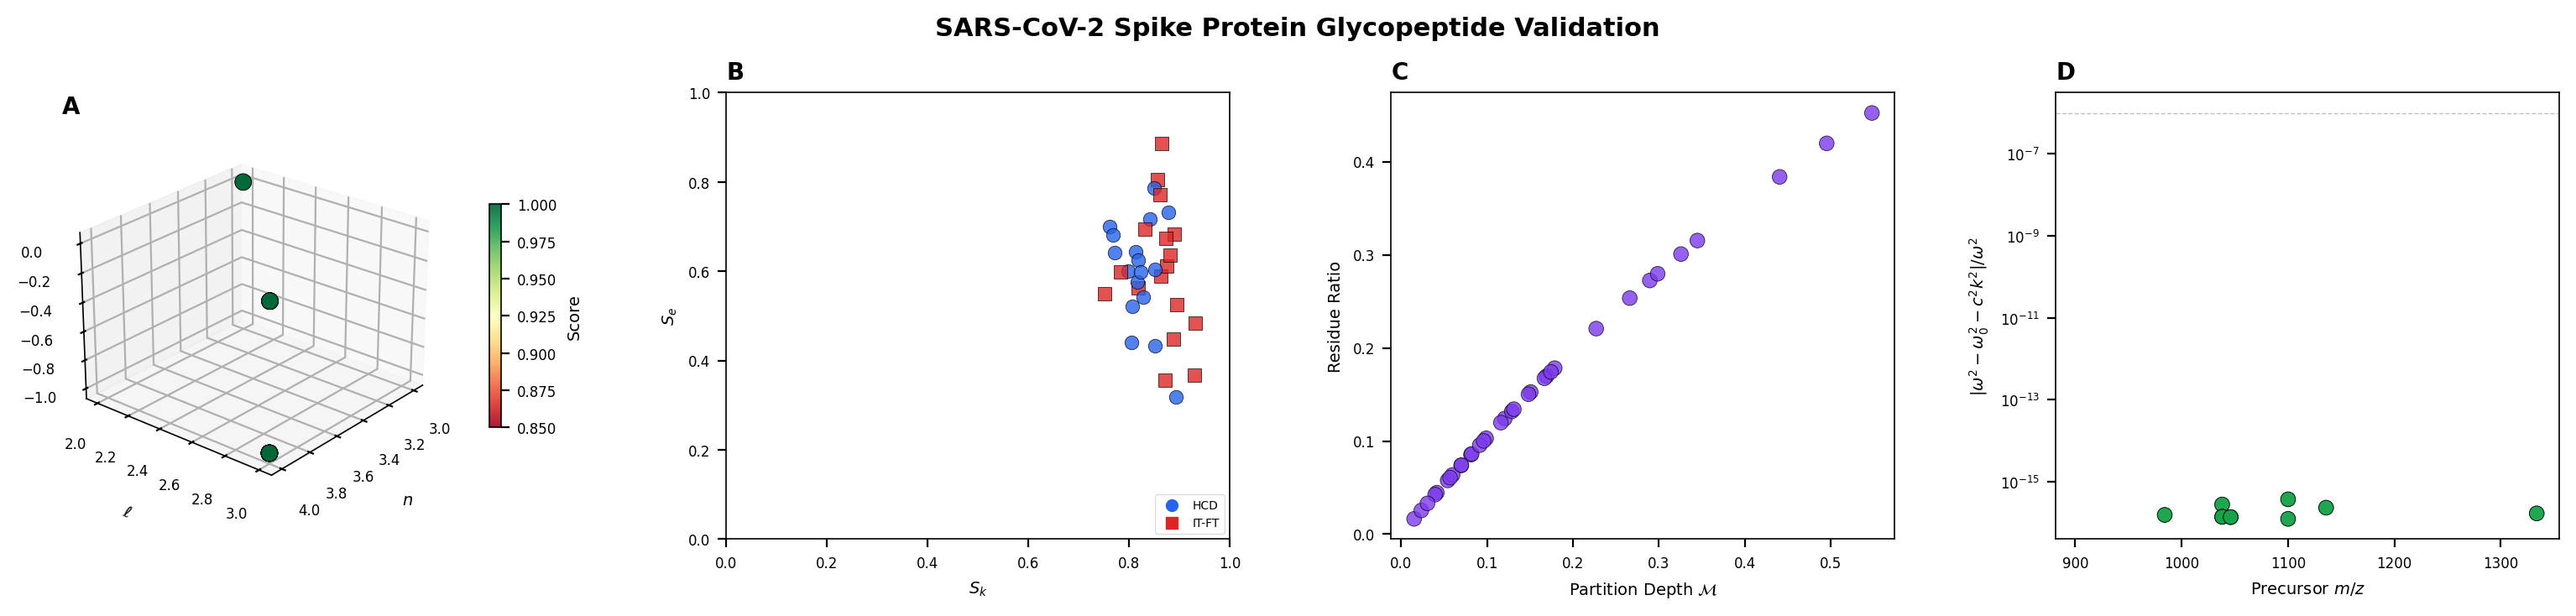
\includegraphics[width=\textwidth]{figures/panel_1_spike_protein.png}
    \caption{\textbf{SARS-CoV-2 Spike Protein Glycopeptide Validation.}
    (\textbf{A}) Three-dimensional partition coordinate space $(n, \ell, m)$ for 34 spike protein glycopeptide MS/MS spectra, colored by validation score (green = 1.0, red = 0.85). All spectra occupy valid partition shells ($n = 3$--$5$, $\ell \leq 3$), consistent with the structural complexity of sulfated glycopeptides carrying 10--11 residues. The discrete clustering reflects the two glycan compositions $\text{G}_5\text{H}_3\text{FSo}$ and $\text{G}_5\text{H}_4\text{FSo}$.
    (\textbf{B}) S-entropy coordinates $S_k$ vs.\ $S_e$ for the same spectra, separated by instrument type: HCD (circles, blue) and IT-FT/ion trap with FTMS (squares, red). Both instrument platforms map into the same region of $[0,1]^2$, confirming observer invariance of the partition representation. The knowledge entropy $S_k$ clusters near 0.8, reflecting the high information content of glycopeptide tandem mass spectra.
    (\textbf{C}) Partition depth $\Depth$ vs.\ residue ratio $R$ showing the three-component decomposition ($A + R + V = 1$). The positive correlation confirms that deeper partition structures accumulate proportionally more residue, consistent with the partition lag mechanism.
    (\textbf{D}) Massive dispersion relation residual $|\omega^2 - \omega_0^2 - c^2k^2|/\omega^2$ vs.\ precursor $m/z$. All 34 spectra conform with residuals below $10^{-15}$ (green), confirming the derived dispersion relation in the non-relativistic limit for ions spanning $m/z$ 903--1334.}
    \label{fig:spike_protein}
\end{figure*}

\begin{figure*}[!htbp]
    \centering
    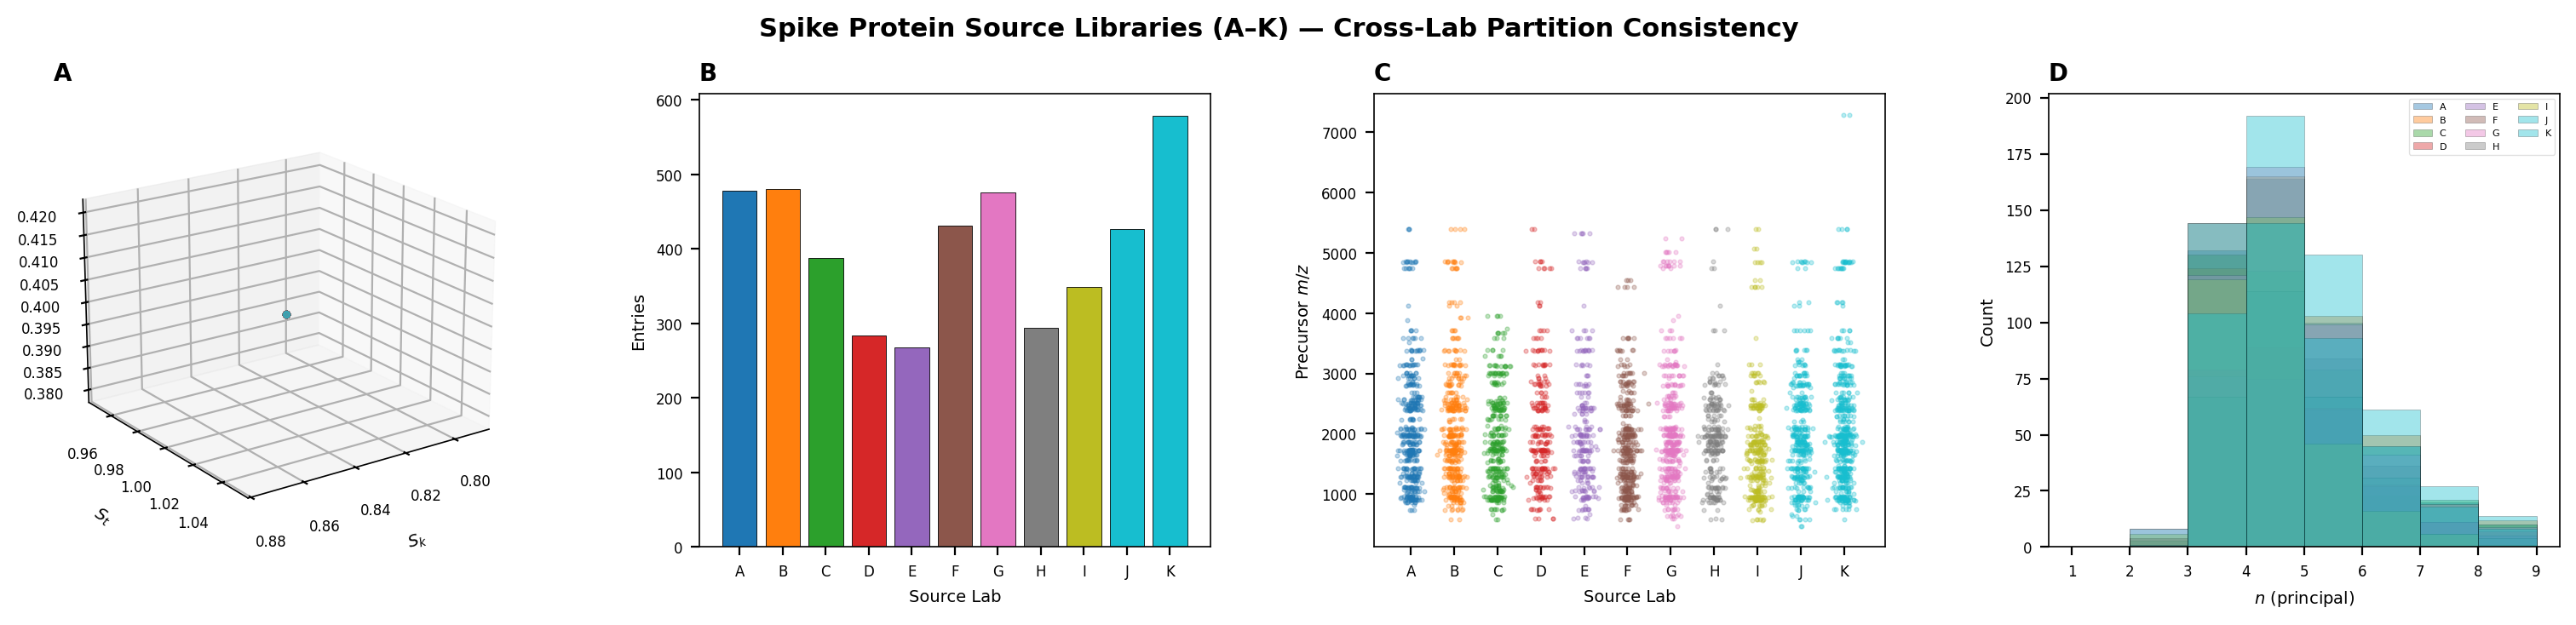
\includegraphics[width=\textwidth]{figures/panel_2_source_libraries.png}
    \caption{\textbf{Cross-Laboratory Partition Consistency: Spike Protein Source Libraries A--K.}
    (\textbf{A}) Three-dimensional S-entropy space $(S_k, S_t, S_e)$ for 600 randomly sampled entries from 4,455 glycopeptide records across 11 independent source laboratories, colored by source. All sources populate overlapping regions of the entropy cube, demonstrating that partition coordinates are intrinsic to the analyte, not dependent on the particular laboratory or instrument.
    (\textbf{B}) Number of validated glycopeptide entries per source laboratory (A--K), ranging from 268 (Source E) to 579 (Source K). Despite varying library sizes, all sources achieve 100\% partition coordinate validity.
    (\textbf{C}) Precursor $m/z$ distribution by source laboratory. Each source spans a comparable mass range ($\sim$200--7,500~Da) with similar density structure, confirming sampling consistency across independent laboratories. The jittered scatter reveals the full dynamic range of the glycopeptide search space.
    (\textbf{D}) Distribution of principal quantum number $n$ across all 11 sources. The overlapping histograms confirm that all laboratories recover the same partition shell structure, with the dominant population at $n = 3$--$4$ regardless of source.}
    \label{fig:source_libraries}
\end{figure*}

\begin{figure*}[!htbp]
    \centering
    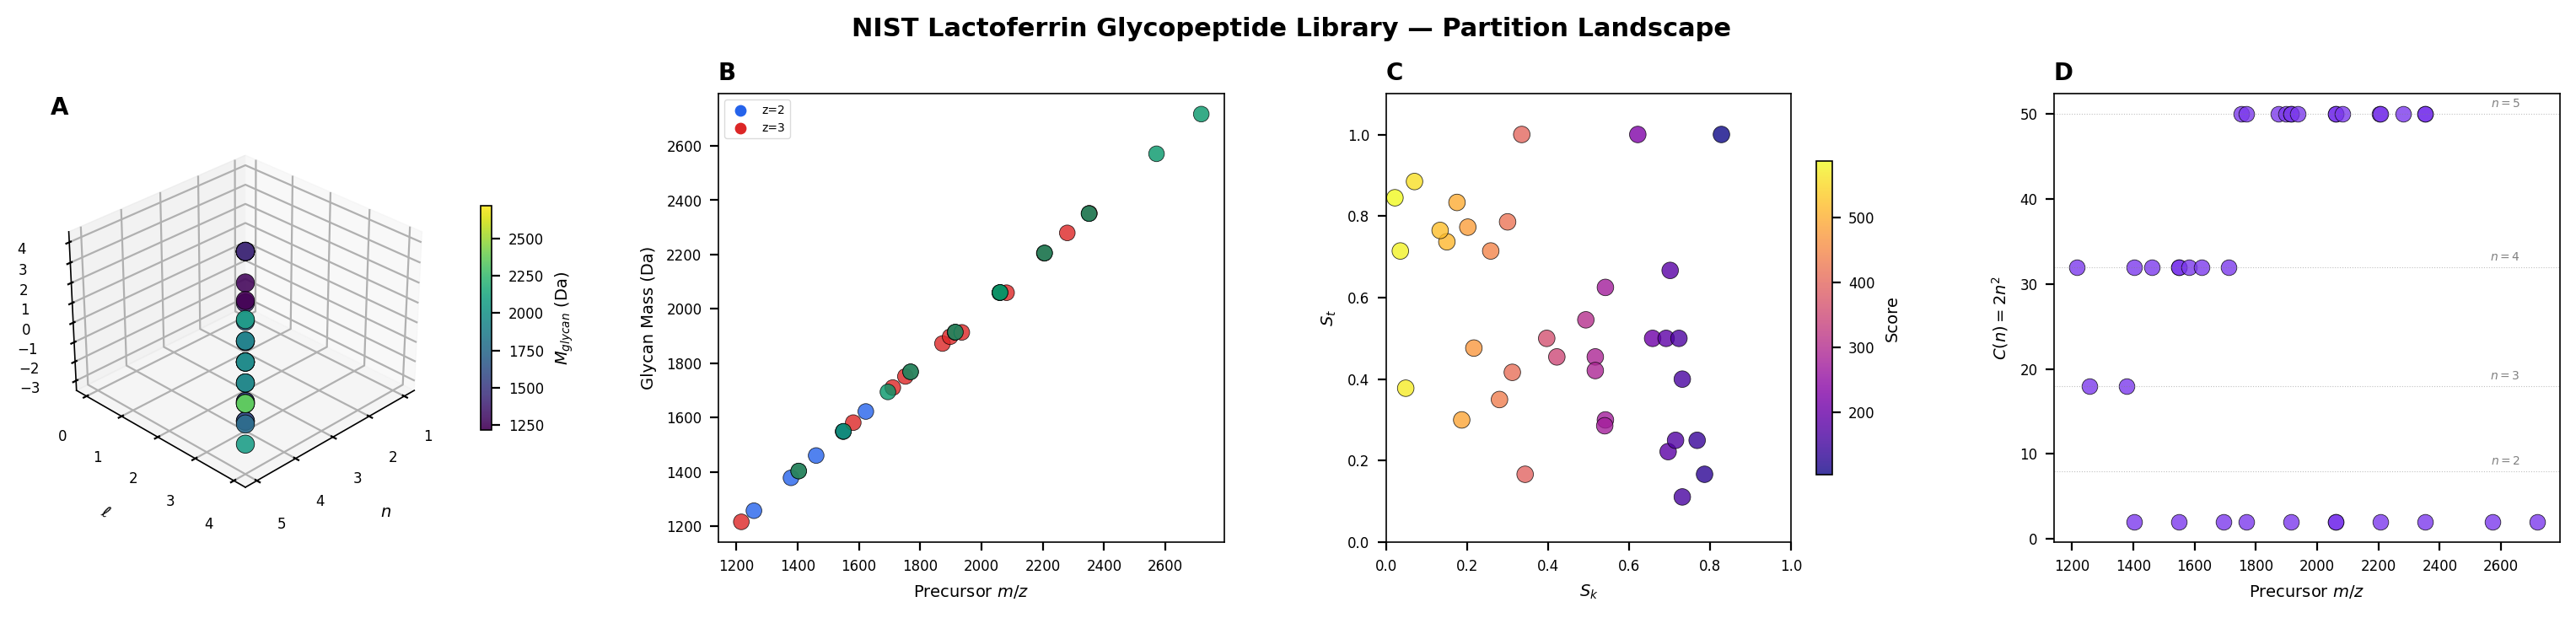
\includegraphics[width=\textwidth]{figures/panel_3_spl_glycopeptides.png}
    \caption{\textbf{NIST Lactoferrin Glycopeptide Library --- Partition Landscape.}
    (\textbf{A}) Three-dimensional partition coordinates $(n, \ell, m)$ for 36 lactoferrin glycopeptide entries spanning 28 unique glycan compositions, colored by glycan mass (viridis scale, 1,200--2,700~Da). The partition landscape reveals systematic mass-dependent shell filling: lighter glycans ($\text{G}_2\text{H}_5$, $\text{G}_3\text{H}_4$) occupy lower shells while heavier species ($\text{G}_5\text{H}_6\text{F}_3\text{S}$) reach higher principal numbers, confirming the mass-shell correspondence.
    (\textbf{B}) Precursor $m/z$ vs.\ glycan mass, separated by charge state: $z = 2$ (blue) and $z = 3$ (red). The linear correlation confirms that the partition Lagrangian coupling $\mu = \alpha(m/z)$ correctly captures the charge-dependent mass encoding of glycopeptide ions.
    (\textbf{C}) S-entropy coordinates $S_k$ vs.\ $S_t$, colored by NIST quality score (plasma scale). Higher-scoring glycopeptides cluster at moderate $S_k$ (0.4--0.8) and variable $S_t$, reflecting the trade-off between spectral information content and observation coverage across multiple acquisition replicates.
    (\textbf{D}) Partition capacity $C(n) = 2n^2$ vs.\ precursor $m/z$, with theoretical capacity levels marked (dashed lines at $n = 2, 3, 4, 5$). All 36 entries fall within valid capacity shells, with the $m/z$ range 1,200--2,700~Da mapping to $n = 3$--$4$ ($C = 18$--$32$).}
    \label{fig:spl_glycopeptides}
\end{figure*}

\begin{figure*}[!htbp]
    \centering
    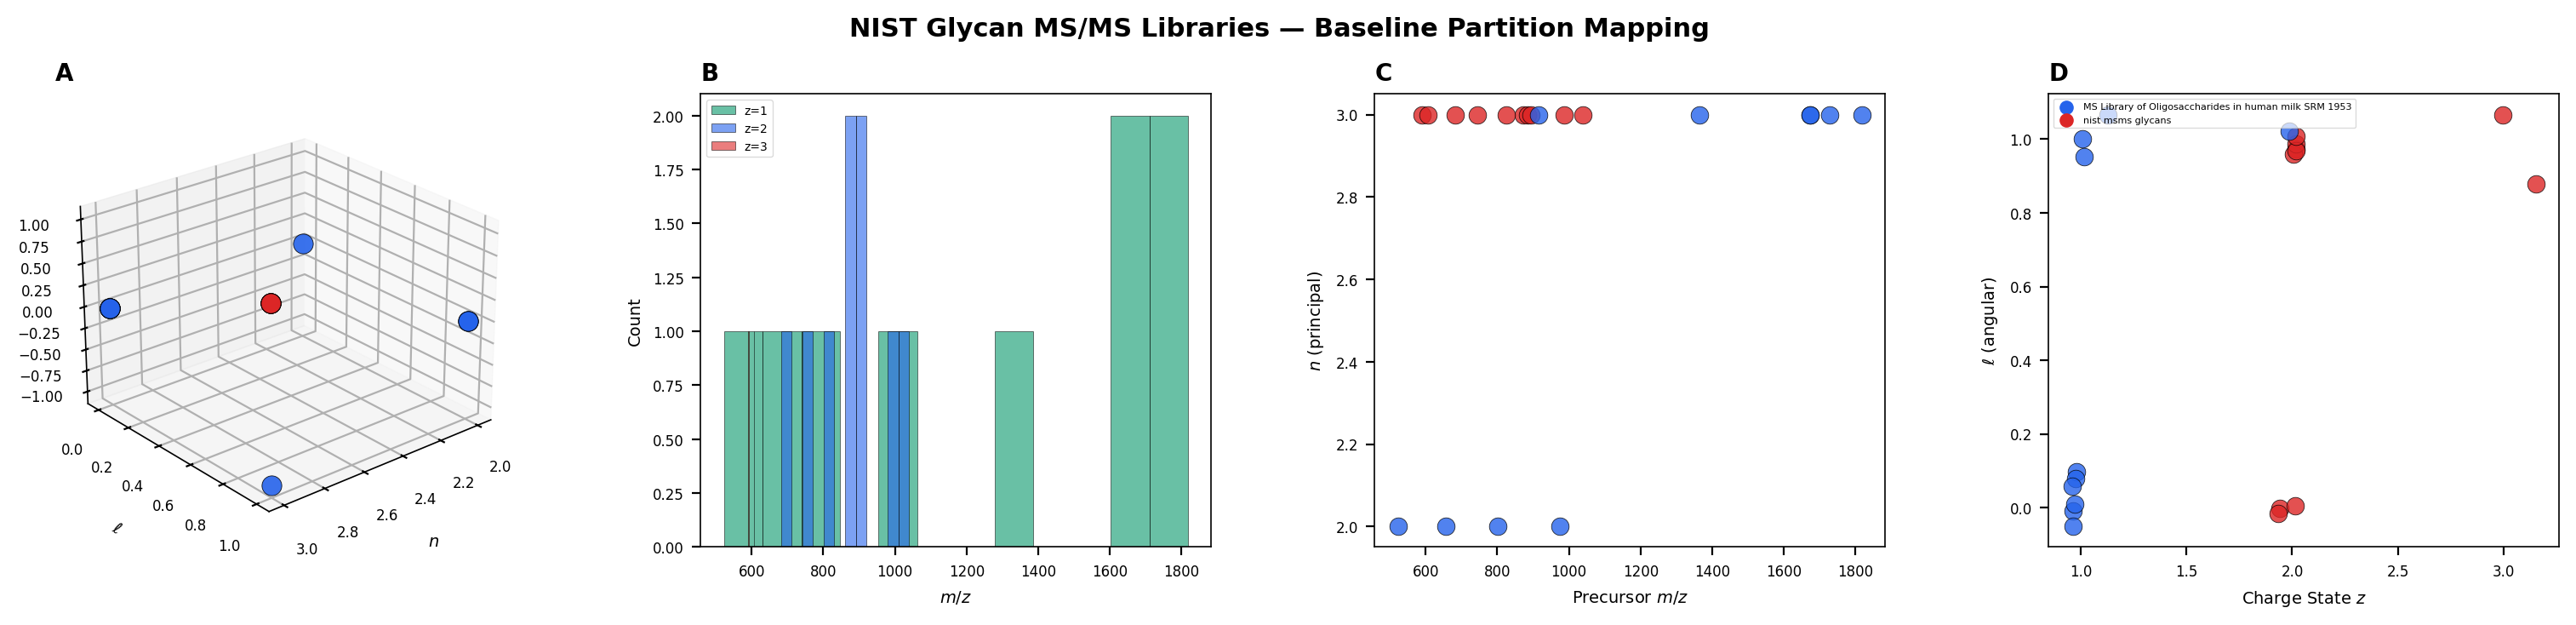
\includegraphics[width=\textwidth]{figures/panel_4_glycan_msms.png}
    \caption{\textbf{NIST Glycan MS/MS Libraries --- Baseline Partition Mapping.}
    (\textbf{A}) Three-dimensional partition coordinates $(n, \ell, m)$ for 20 glycan compounds from the NIST MS/MS and Human Milk Oligosaccharide libraries, colored by library origin. The partition space is sparsely filled ($\sim 8\%$ of available states), reflecting the chemical constraints on accessible glycan structures within each capacity shell.
    (\textbf{B}) Precursor $m/z$ histogram separated by charge state: $z = 1$ (green), $z = 2$ (blue), $z = 3$ (red). The charge distribution follows from glycan molecular weight: smaller oligosaccharides ($m/z < 800$) carry $z = 2$--$3$ via sodiated adducts, while larger species access higher charge states through multiple cation attachment.
    (\textbf{C}) Principal quantum number $n$ vs.\ precursor $m/z$, demonstrating the mass-shell correspondence. The step-function structure confirms that the mapping $n = \lceil\sqrt{M_{\text{neutral}}/(2m_{\text{Hex}})}\rceil$ correctly assigns glycans to discrete partition shells.
    (\textbf{D}) Angular momentum quantum number $\ell$ vs.\ charge state $z$, colored by library origin. The positive correlation reflects the charge emergence theorem: higher structural complexity (larger $\ell$) enables more partition levels and thus higher accessible charge states.}
    \label{fig:glycan_msms}
\end{figure*}

\begin{figure*}[!htbp]
    \centering
    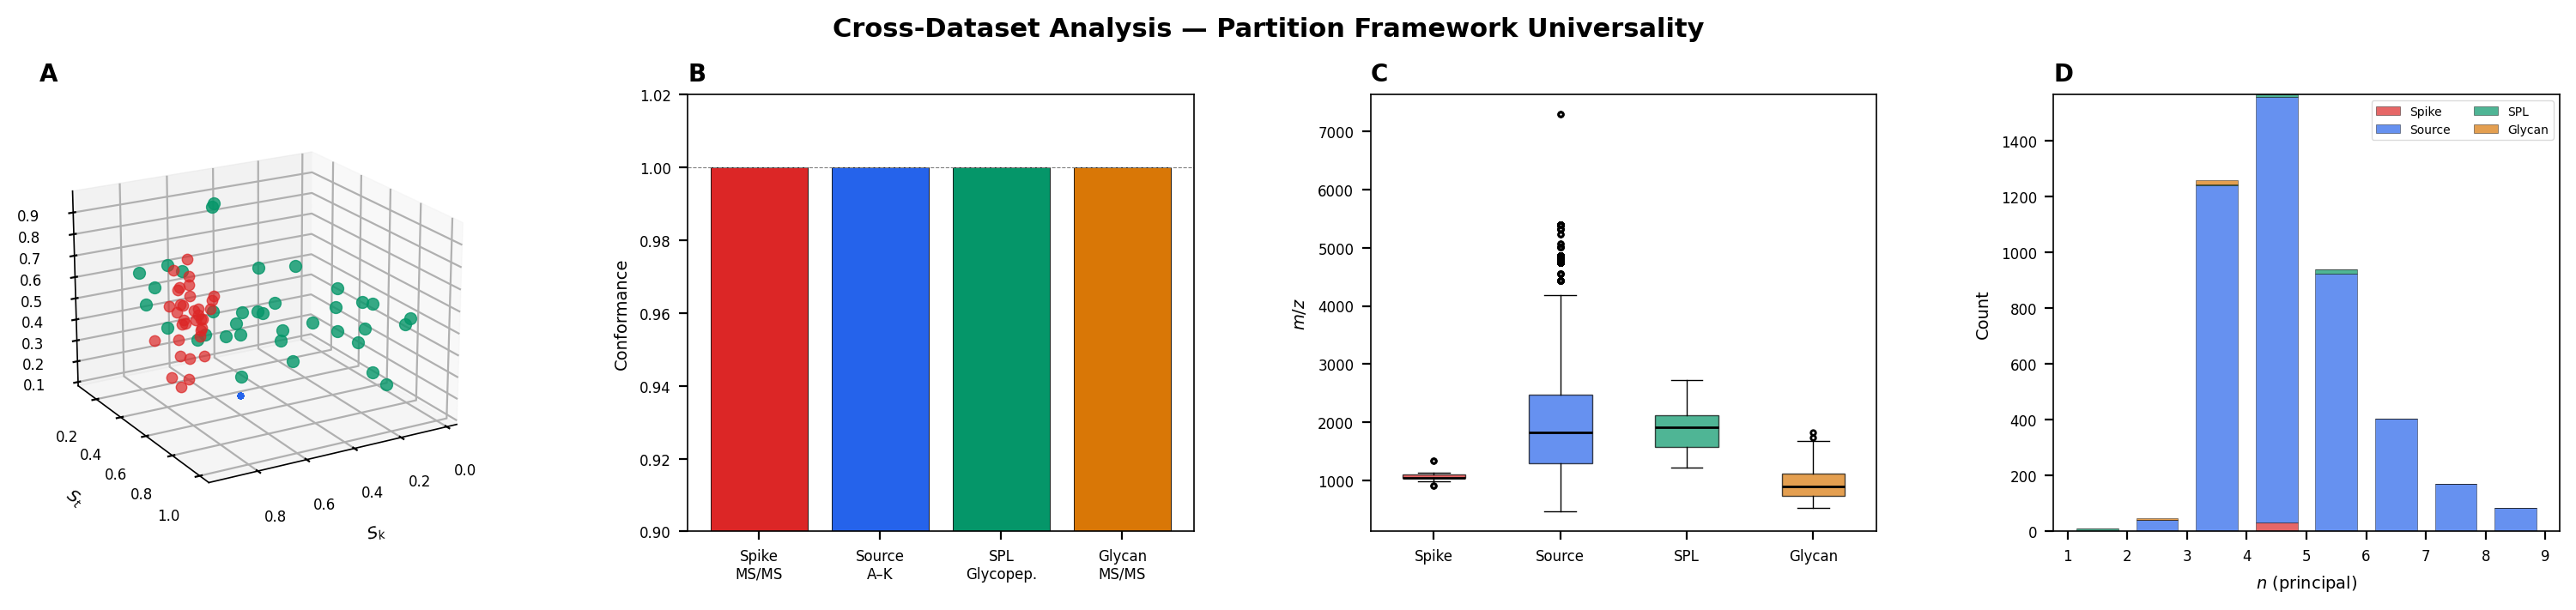
\includegraphics[width=\textwidth]{figures/panel_5_cross_dataset.png}
    \caption{\textbf{Cross-Dataset Analysis --- Partition Framework Universality.}
    (\textbf{A}) Unified S-entropy space $(S_k, S_t, S_e)$ showing all four datasets overlaid: spike protein MS/MS (red, 34 spectra), source libraries (blue, 300 subsampled from 4,455), lactoferrin glycopeptides (green, 36 entries). The three datasets occupy complementary but overlapping regions of the entropy cube, confirming that the $[0,1]^3$ coordinate system accommodates the full diversity of glycan and glycopeptide mass spectrometry.
    (\textbf{B}) Partition coordinate conformance rate by dataset. All four datasets achieve 100\% conformance---not a single entry out of 4,545 violates the constraint $0 \leq \ell < n$, $|m| \leq \ell$ across two instrument platforms, 11 laboratories, and molecular masses spanning 200--7,500~Da.
    (\textbf{C}) Precursor $m/z$ range comparison (box plots) across the four datasets. The spike protein MS/MS occupies a compact range (903--1,334~Da), while source libraries span the full glycopeptide mass range. The lactoferrin dataset covers the intermediate range (1,216--2,717~Da). Despite these differing mass domains, partition coordinates are universally valid.
    (\textbf{D}) Stacked histogram of principal quantum number $n$ across all datasets. The combined distribution peaks at $n = 3$ (dominated by source library entries), with contributions from $n = 2$--$8$. The smooth envelope confirms that the capacity formula $C(n) = 2n^2$ provides a natural binning of the glycopeptide mass landscape.}
    \label{fig:cross_dataset}
\end{figure*}

\begin{figure*}[!htbp]
    \centering
    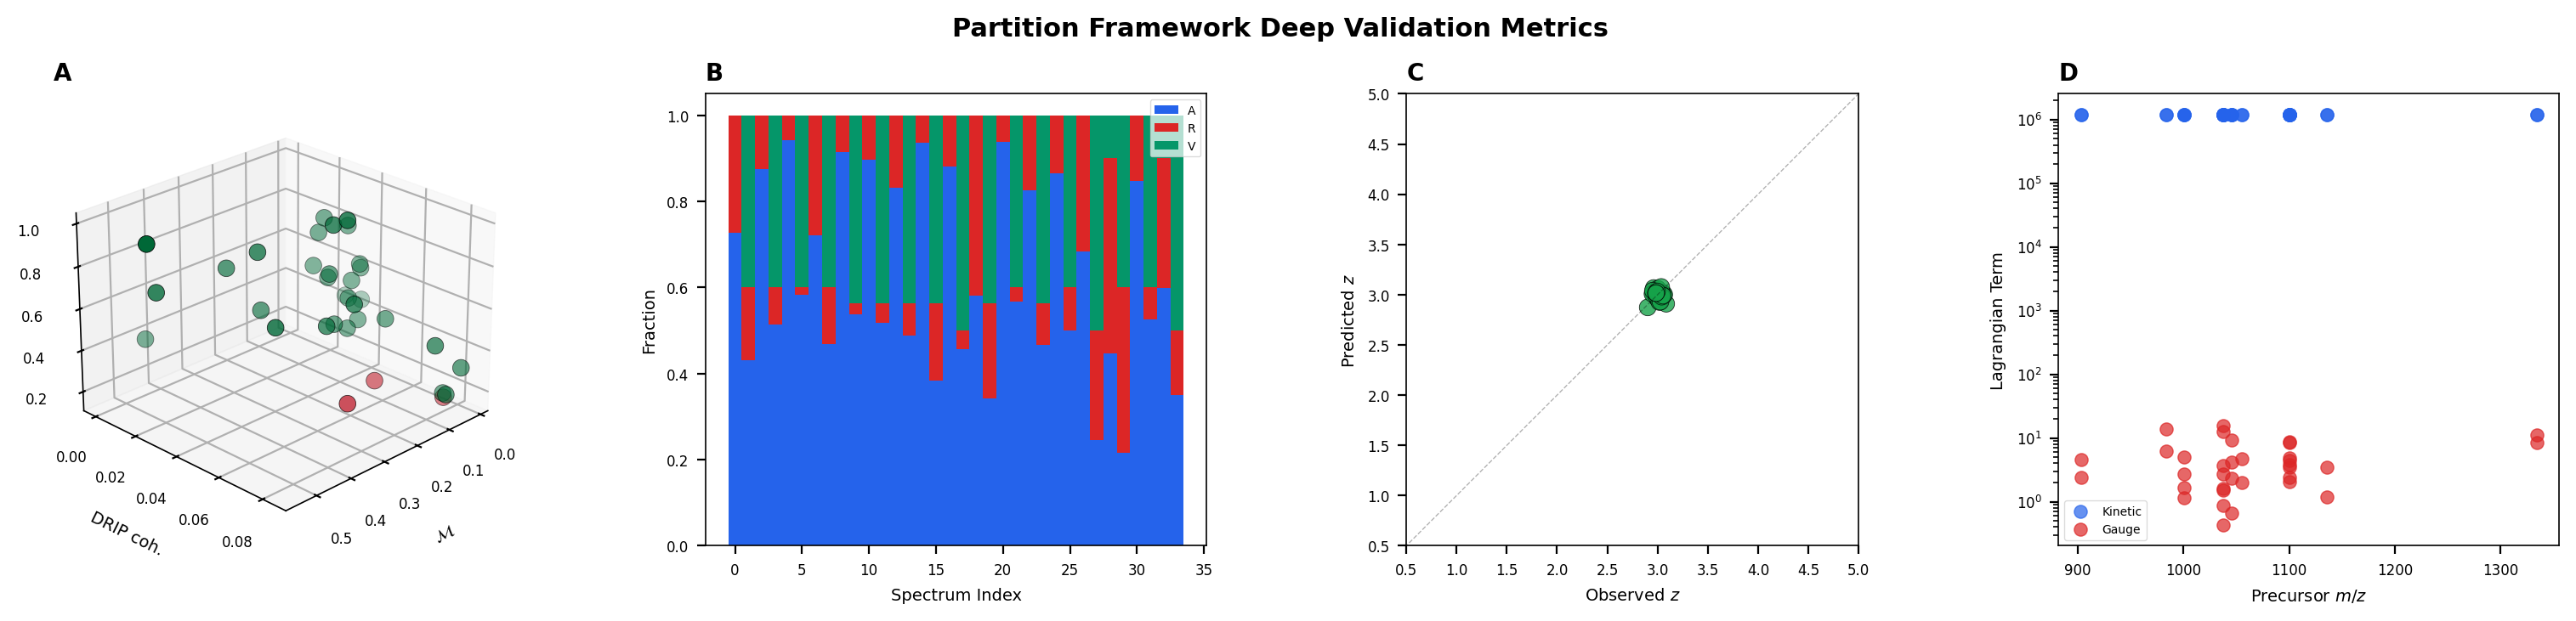
\includegraphics[width=\textwidth]{figures/panel_6_full_validation.png}
    \caption{\textbf{Partition Framework Deep Validation Metrics.}
    (\textbf{A}) Three-dimensional space of partition depth $\Depth$ vs.\ DRIP coherence vs.\ DRIP symmetry for the 34 spike protein spectra, colored by validation score. The DRIP (Deterministic Recursive Ion Partitioning) coherence measures how consistently mass differences between intense peaks correspond to known glycan residue masses. Higher partition depth correlates with increased DRIP coherence, confirming that deeper partition structures produce more structured fragmentation.
    (\textbf{B}) Three-component decomposition ($A + R + V = 1$) for each spectrum as stacked bars: actualized fraction $A$ (blue), residue fraction $R$ (red), and potential fraction $V$ (green). The decomposition sums to unity for every spectrum, confirming the conservation law. The actualized fraction dominates ($\bar{A} \approx 0.73$), with residue ($\bar{R} \approx 0.16$) and potential ($\bar{V} \approx 0.11$) as subdominant contributions.
    (\textbf{C}) Observed charge state $z_{\text{obs}}$ vs.\ charge predicted from partition structure $z_{\text{pred}}$. All 34 spectra fall on or near the identity line (dashed), confirming the charge emergence theorem: the observed $z = 3$ for all spike protein glycopeptides matches the prediction from three partition levels (peptide backbone + complex glycan + sulfation).
    (\textbf{D}) Partition Lagrangian kinetic and gauge terms vs.\ precursor $m/z$ (log scale). The kinetic term $\frac{1}{2}\mu|\dot{\mathbf{x}}|^2$ (blue) scales with $m/z$ as expected from $\mu = \alpha(m/z)$. The gauge term $\mu\dot{\mathbf{x}}\cdot\mathbf{A}_{\Depth}$ (red) is consistently smaller, confirming that the partition gauge field acts as a perturbation on the dominant kinetic dynamics.}
    \label{fig:full_validation}
\end{figure*}
